\section{Implementation}

In this section we give algorithms of some important functions of our work that will complement the understanding of previous chapter.

\subsection{Main method}
Although the actual implementation has been done in $C++$ using object oriented concepts (different classes) however for the sake of simplicity implementation in this document is only based on functions and some local and global variables that need be passed to these functions.

The algorithm \ref{al:general} implements the main function that has the controling loop and calls appropriate functions to realize the complete motion detection logic.

%In the Algorithm \ref{al:general}, we provide an overview of the framework created for detecting moving parts.

\begin{lstlisting}[title={Algorithm},mathescape=true,label=al:general,caption={Main algorithm for motion detection}]
//Global Variables
//Some data structures
//  Structure to keep motion data given by MTi-G motion sensor installed on the vehicle
struct MotionData { $timestamp$, $velocity_x$, $velocity_y$, $quaternion \{q0,q1,q2,q3\}$ }
//  Structure for processed motion data (considered as control data)
struct U { $speed$, $angular$_$speed$, $dt$ }
//  Structuer for pose
struct Pose { $x$, $y$, $\theta$}
//  Structure for cell in grid
struct Cell { $row$, $col$ }
//Total cells of the occupancy Grid
N //of type int
//New Occupancy Grid given by the laser fusion module
$OG_t$[N] //of type float
//Occupancy Grid for last time step (t-1)
$OG_{t-1}$[N] //of type float
//Arrays to keep count of occupied counts for each cell
//  Occupied Counts for current data at time t
$OC_t$[N] //of type int
//  Accumulated counts until time t-1
$OC_{t-1}$[N]  //of type int
//Arrays to keep count of free counts for each cell
//  Free Counts for current data at time t
$FC_t$[N]  //of type int
//  Accumulated counts until time t-1
$FC_{t-1}$[N] //of type int
//Variables to keep current and last motion data
$MotionData_t$  //of type MotionData
$MotionData_{t-1}$  //of type MotionData
//Processed motion data
$u_t$ //of type U
//Results array
$MotionGrid$[N] //of type float

//Main controlling method
DetectMotion() 
	//Initialize global variables
	InitGlobalVars () (*@\label{ln:InitGlobalVars}@*)
	//Main loop
	while not quit do 
		//Get occupancy grid from current laser data, Fusion module prepares this grid
		$OG_t$ = ReadAndFuseLaserData() (*@\label{ln:ReadAndFuseLaserData}@*)
		//Get new raw motion data from the sensor (from Hugr store)
		$MotionData_t$ = ReadMotionData() (*@\label{ln:ReadMotionData}@*)
		//Calculate control data (motion) from current and last raw motion data
		$u_t$=FindMovement()
		//Initialize counter arrays from new data
		InitCounterArraysForNewData()
		//Upate counter arrays from accumulated counts until time step t-1
		UpdateCounterArrays($u_t$)
		//Calculate final motion grid
		CalculateMotionGrid()
		//at this point $MotionGrid$ has the results
		//Save updated values for next step
		$OG_{t-1}$=$OG_t$
		$MotionData_{t-1}$=$MotionData_t $
		$OC_{t-1}$=$OC_t$
		$FC_{t-1}$=$FC_t$
	
\end{lstlisting}
This is the outline of the main function to detect motion from laser data. The function\\ $InitGlobalVars()$ at line number \ref{ln:InitGlobalVars} initializes the global variables with logical values. The function  $ReadAndFuseLaserData()$ at line \ref{ln:ReadAndFuseLaserData} has been implemented by another member of the team and is based on the technique published in \cite{ADARVE-2012-671211}. $ReadMotionData()$ function at line \ref{ln:ReadMotionData} simply reads raw motion data from the sensor (actually from the middleware Hugre store). Rest of the functions are outlined below.

%The elements from the Algorithm \ref{al:general} are defined in the high level of abstraction. In the next sections we are going to explain the calls made in this code.

%All variables declared out of the function scope are considered as global variables, but for better understanding of the dependencies among the functions, the input data are going to be sent by parameter in some situations.

\subsection{Finding the movement}
The listing in algorithm \ref{al:movement} gives the logic of method $FindMovement()$ used to calculate $u_t$.
\begin{lstlisting}[label=al:movement,mathescape=true,caption={Find the movement of the vehicle}]
FindMovement()
	//local variables
	$velX, velY$ //of type float
	$yaw, yaw2$ //of type float
	$Q$ //of type quaternion
	//velocity vector from horizontal and vertical speed components
	$velX=MotionData_t.velocity_x$
	$velY=MotionData_t.velocity_y$
	$u_t.speed=$sqrt$(velX*velX+velY*velY)$
	
	//quaternion to euler angles conversion	
	$Q=MotionData_t.quaternion$
	$yaw=$atan2$(2(Q.q0*Q.q3+Q.q1*Q.q2),1-2(Q.q2*Q.q2+Q.q3*Q.q3))$	

	$Q=MotionData_{t-1}.quaternion$
	$yaw2=$atan2$(2(Q.q0*Q.q3+Q.q1*Q.q2),1-2(Q.q2*Q.q2+Q.q3*Q.q3))$	
	
	$u_t.dt=MotionData_t.timestamp-MotionData_{t-1}.timestamp$
	
	$u_t.angular$_$speed=(yaw2-yaw)/u_t.dt$
	
	return $u_t$
\end{lstlisting}

%This algorithm is used to calculate the $u_t$, mathematically explained previous sections, $u_t$ 

\subsection{Initializing Grid from new data}

\begin{lstlisting}[label=al:initializeGrid,mathescape=true,caption={Initialization of the grid}]
InitCounterArraysForNewData()
	for $i=0$ to $N-1$ do
		if $OG_t[i] > 0.5$ then 
			$OC_t[i]=1$
			$FC_t[i]=0$
		else if $OG_t[i] < 0.5$ then
		
			$OC_t[i]=0$
			$FC_t[i]=1$
		else
			$OC_t[i]=0$
			$FC_t[i]=0$
\end{lstlisting}

This listing \ref{al:initializeGrid} initializes the counters (occupied and free) based on the information available in the current Occupancy Grid $OG_t$.

\subsection{Updating Counter arrays}

\begin{lstlisting}[label=al:updatecounter,mathescape=true,caption={Update counter arrays}]
UpdateCounterArrays()
	//local variables
	$newPose, invPose$ //of type Pose
	$P_i, P_j$ //of type Pose
	$cell_i, cell_j$ //of type Cell
	$i, j$ //of type int
	//Find pose of new grid $OG_t$ w.r.t old grid $OG_{t-1}$
	$newPose$=FindPoseOfNewGrid($u_t$)
	//Find inversepose, i.e pose of $OG_{t-1}$ w.r.t $OG_t$
	$invPose$=FindInversePose($newPose$)
	//Loop on all cells in grid $OG_{t-1}$ to find their position in grid $OG_t$
	//These transformations essentially map a cell $i$ in grid $OG_{t-1}$ to a cell $j$ in $OG_t$
	for $i=0$ to $N-1$ do
		//ith cell in grid $OG_{t-1}$
		$cell_i$ = CellFromIndex($i$)
		//pose of cell in grid: x,y coordinates of the center of the cell
		$P_i$=PoseOfCell($cell_i$)
		//pose of cell $i$ of grid $OG_{t-1}$ in grid $OG_t$
		$P_j$=CompoundPose($invPose$,$P_i$)
		//cell where point $P_j$ lies in the grid
		$cell_j$=CellFromPose($P_j$)
		If $cell_j$ is not visible in $OG_t$ then
			continue
		$j$ = IndexFromCell($cell_j$)
		$OC_t[j]+=OC_{t-1}[i]$
		$FC_t[j]+=FC_{t-1}[i]$
\end{lstlisting}
The listing \ref{al:updatecounter} explaines how to map a cell from $OG_{t-1}$ to $OG_t$ and update the counter arrays. Some of the functions will not be detailed, specifically those in which the translation between mathematical and algorithms perspective do not change considerably.
The function $FindPoseOfNewGrid()$ simply implemments the Equation~\ref{eq:circularmotion}. $CompoundPose()$ and \\$FindInversePose()$ functions implement the equation \ref{eq:composepose} and \ref{eq:invpose}  respectively. $CellFromPose()$ is mapped from Equation~\ref{eq:grid:cell:calculation} whereas $PoseOfCell()$ is exactly inverse of $CellFromPose()$. Functions $CellFromIndex()$ and $IndexFromCell()$ map 1D array to 2D array and vice versa respectively.

\begin{lstlisting}[label=al:motiongrid,mathescape=true,caption={Calculate motion grid}]
CalculateMotionGrid()
	//loop on all grid cells and classify them as static or moving
	for $i=0$ to $N-1$ do
		$MotionGrid[i]=0$
		if $OG_t[i] > 0.5$ and $FC_t[i] > 2*OC_t[i]$ then
			$MotionGrid[i]=1$
\end{lstlisting}

Listing \ref{al:motiongrid} implements a simple decision function based on current vale of the cell and the two counter values to decide if it belongs to a moving object or not.

\section{Experiments And Results}

%In the experimentation phases, we modeled the algorithm to compute ahead of the time by using the bicycle model and extrapolating the pose by using the current vehicle measurements, like stearing angles. But this measurement had shown a lot of variation during a run, and the extrapolated model gets out to date very quickly.

%From mechanical physics we obtain the angular velocity and from the vehicle \emph{CAN bus} we obtain the data time stamp, and along with it the time variation, $\Delta t$.

%Using transformational matrices we bring the car perspective \cite{iyengar1991autonomous} and the prediction to the same frame of reference.

%\section{Evaluation}

%target: dynamic and static separation, reduce the number of frames required, no classification, no association; no tracking, no 

\subsection{Testbed}
\label{sec:testbed}

%\subsubsection*{Hardware}
Experiments for this work have been done on data sets from a Lexus LS600h demonstrator vehicle equipped with a stereo vision camera (TYZX), two IBEO Lux Lidar scanners and a MTi-G XSens IMU+GPS sensor. Onboard processing unit is a 4 core Dell workstation with a NVidia GPU graphic card to do parallel processing. This hardware setup is shown in figures \ref{fig:Lexus} and \ref{fig:Lexus2}. Some details of our main sensors (Lidar and MTi-G) are given in last chapter.
%For testing purposes, we have a Lexus LS600h equipped with a stereo vision (TYZX camera) positioned in the superior part of the windshield.

%The vehicle has two IBEO Lux Lidar in the front side of the car, one in each corner of the bumper.

%As IMU, the car is equipped with a Xsens IMU and a GPS for global positioning.

\begin{figure}[h]
   \centering
     \begin{tabular}{lr}
     \multicolumn{2}{c}{ 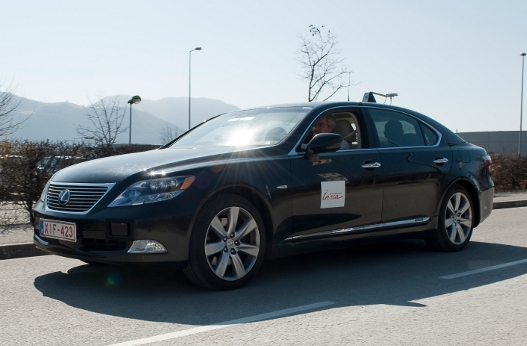
\includegraphics[width=0.55\columnwidth]{img/testbed:car}}\\
       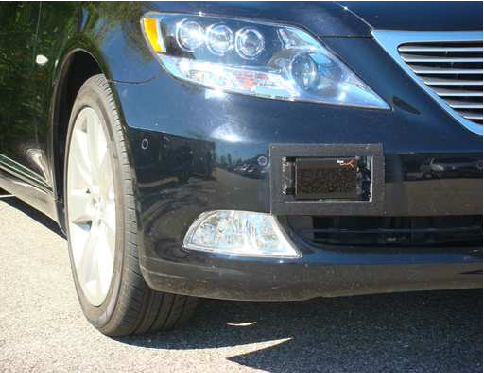
\includegraphics[width=0.40\columnwidth]{img/testbed:ibeo}
       &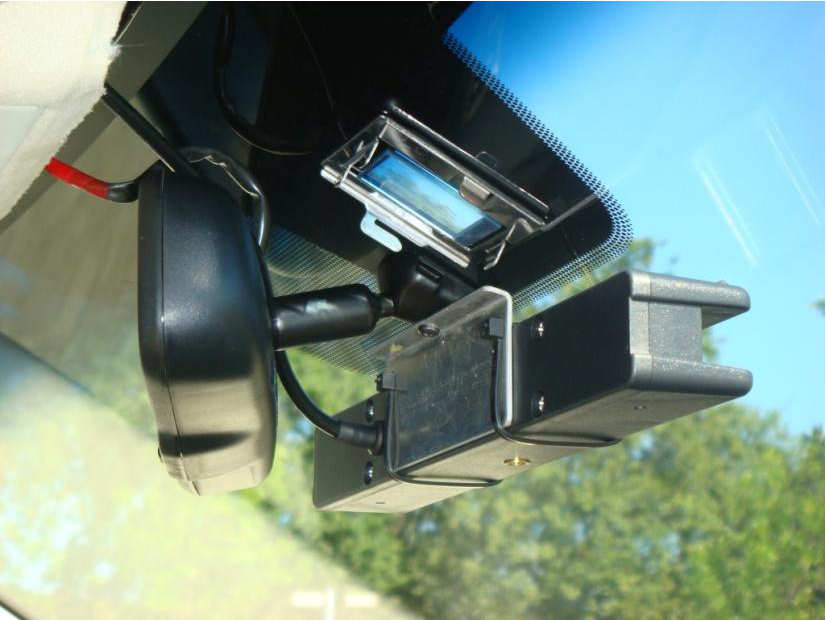
\includegraphics[width=0.40\columnwidth]{img/testbed:tyzx}
     \end{tabular}
   \caption{Lexus LS600h car equipped with two IBEO Lux lidars and a TYZX
     stereo camera}
   \label{fig:Lexus}
 \end{figure}

%As the test platform requires a powerfull computer to process the stereo images in realtime, the car is equipped with a Dell workstation with an NVidia graphic card.

%DeepSea TYZX stereo vision camera has a base line of 22 cm with 512x320 pixels of resolution and focal length of 410 pixels, this camera is provided with a library which can estimate the distance in cm of the objects captured by the camera, but in our tests we used the estimators developed at Inria\cite{PERROLLAZ-2010-493397}.
%better references
%http://ieeexplore.ieee.org/stamp/stamp.jsp?tp=&arnumber=6170895
%http://hal.inria.fr/index.php?halsid=fa9c2loot97ptftt2n38f6lvr5&view_this_doc=hal-00671208&version=1

\begin{figure}[h]
   \centering
     \begin{tabular}{lr}
       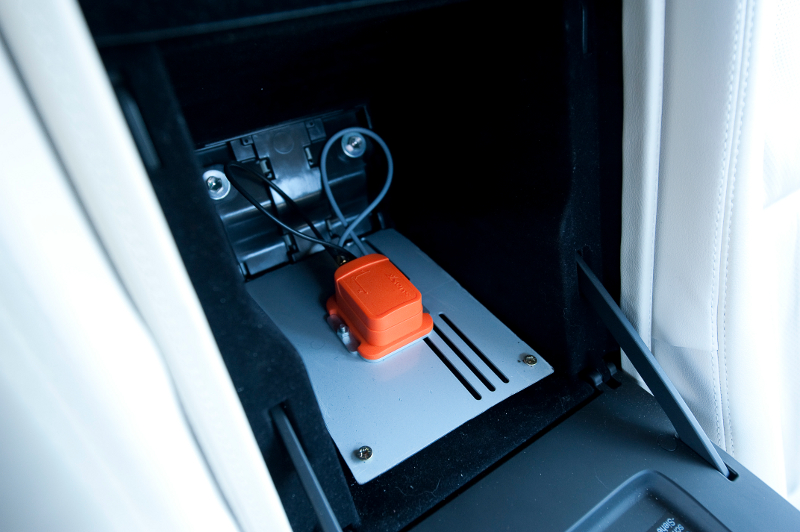
\includegraphics[width=0.45\columnwidth]{img/testbed:xsens}
       & 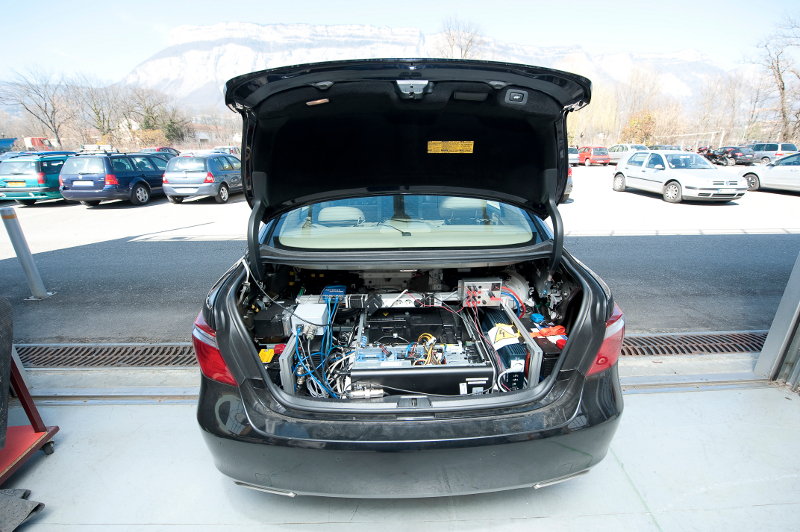
\includegraphics[width=0.45\columnwidth]{img/testbed:trunc}
     \end{tabular}
   \caption{MTi-G XSens IMU unit \& Intel Xeon 3.4GHz linux box}
   \label{fig:Lexus2}
 \end{figure}

%Each IBEO Lux Lidar is composed of four layers, each of them providing about 200 beams. The angular range of 100 degrees with angular resolution of 0.5 degrees. Each beam can reach until 200 m of distance measurement, with width of 40 m and maximum height of 2 m.

%MTi-G XSens minimum of 120Hz and maximum of 512Hz for data logging and angular resolution of 0.05 degrees, all specifications are valid when considering an homogenous eletromagnetic environment. Maximum altitude operation is 18 Km and maximum speed is 515 m/s.



\subsection{Middleware Software}

The robotic cars are equipped with different types of communication layers which are responsible for information sharing between different components. A commonly used communication technique is known as Controller Area Network (CAN) that provides a cheap and reliable way to communicate with devices.%, so CAN bus have been replacing the regular point-to-point wiring interconnection among the components\cite{bosch91can}.

Since data sharing is a critical part of a robotic system some standards have started to appear in this field. Like Data Distribution Service\cite{dds} is a set of specifications for data distribution in real-time systems, this specification is maintained by OMG Data Distribution SIG (DDSIG).

DDS works in a publish-subscriber manner, where the subscriber acquire the data by subscribing to one or several  "topics", which is the name assigned for a data provider (the publisher itself). The goal is to promote the lose coupling and real-time data sharing between applications.

Car manufacturers use platforms like YARP (Yet Another Robot Platform),  URBI \cite{urbi} or Robot Operating System(ROS) \cite{ros} to publish the information gathered from the sensors and processing modules, frameworks like ROS, allow the car to publish information  which can be accessed by other applications.%, the intent for most of those frameworks is to give longevity\cite{Fitzpatrick:2008:TLR:1327539.1327705} for the robot application that uses it by providing a platform that can evolve in cooperation manner with other projects.
Our demonstrator vehicle uses HugrStore(link?) software middleware to share data between different hardware and software components.

%For this project Robot Operating System(ROS) was adopted, ROS gives us the hability to save all information obtained during a run (driving the test platform) from all sensors, and replay it later in the laboratory, this by far allow to have a consistent test samples and a historical evolution of all scenarios gathered during the algorithm evolution, alowing the retro-performance benchmarking with other versions of the algorithm.

\subsubsection*{HugrStore}
HugrStore is a middleware that allows sharing information among applications using a shared memory segment, in a publisher-subscriber manner. Hugr is DDS compliant. The communication model is represented in the Figure \ref{fig:dds:hugr}. So publisher wirtes a data about a topic in the shared memory that can be read by any subscriber to that topic.

\begin{figure}[H]
   \centering
     \begin{tabular}{lr}
       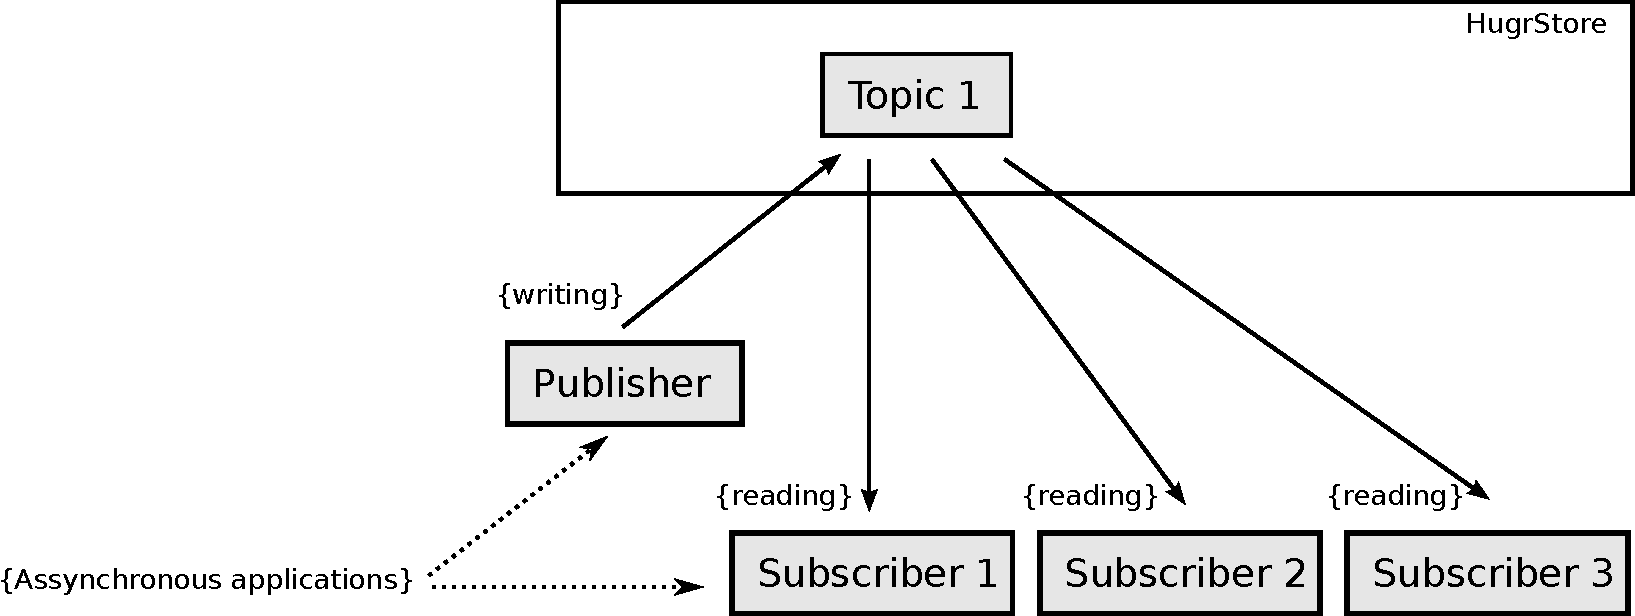
\includegraphics[scale=0.50]{img/fig:dds:hugr}
     \end{tabular}
   \caption{Publisher-Subscriber scheme}
   \label{fig:dds:hugr}
\end{figure}

\subsubsection*{Data Sets}
Data sets for this work have been captured for some urban and highway driving scenarios.

\subsection{Results}

Our algorithm was tested in the XP platform. Different scenarios were collected to assess our method.

In this section, we are going to present the results in a same fasion for different scenarios. In the Figure~\ref{fig:result:framework} we can see three regions in the image, individually each region will be dedicated to display the data in a specific format. We are going to nominate those regions as North, East and West part. 

The \textbf{North} is located in the upper part of the image and will display a snapshot of the footage during a run in the XP platform, this image is a non processed image, obtained directly from the vehicle's camera. \textbf{West} contains the occupancy grid image generated from the North image, and it is located on the left part of the image.

On the \textbf{East} region, we present the resulting image from the \textit{Motion detection module}, which uses West part as input.

\begin{figure}[H]
   \centering
     \begin{tabular}{lr}
       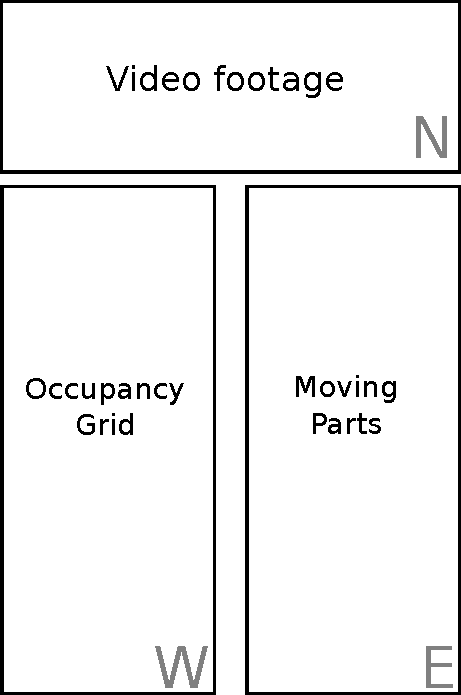
\includegraphics[scale=0.60]{img/fig:result:framework}
     \end{tabular}
   \caption{Presentation of the tests in XP Platform}
   \label{fig:result:framework}
\end{figure}

\subsubsection{Two vehicles at low speed}

In this scenario, the XP platform is performing a soft curve to the right, while two other vehicles are approaching in the opposite direction. The distinction between those vehicles and the enviroment can easily be done on the East part, where the two vehicles are depicted more distinctively.

One vehicle cannot be seen clearly on the North image due to the reflection on the windshield and the trees behind the vehicle which reduces the contrast between the car and the landscape background. Although it can be easily tracked from the East part. We see that these moving vehicles have been detected successfully, the rectangle segmenting the cars have been drawn manually.

\begin{figure}[H]
   \centering
     \begin{tabular}{lr}
       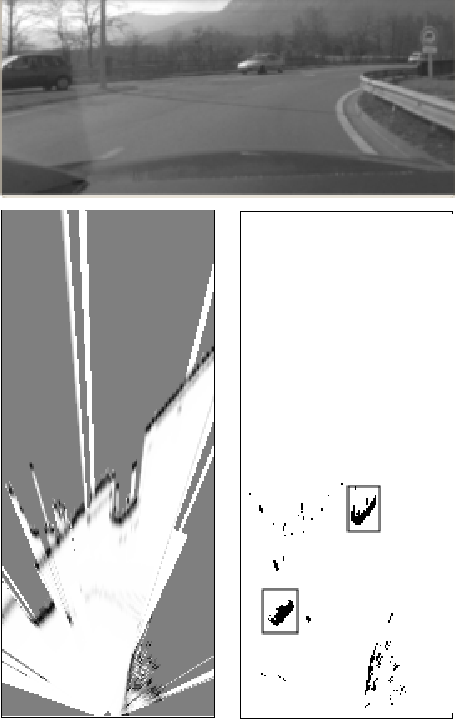
\includegraphics[scale=0.60]{img/fig:result:scenetwocars}
     \end{tabular}
   \caption{Opposite direction vehicles}
   \label{fig:result:scenetwocars}
\end{figure}

\subsubsection{Vehicle in a roundabout}

This scenario is shown in the Figure~\ref{fig:result:scenetwocarrondepoint}. A second vehicle is performing the roundabout, in the East image this vehicle. It can be detected by finding the most significant amount of agglomerated black dots. As we can see from the East part, at short distance we have some noisy, few black dots. But even with those noises we can distinguish a large object moving and a noise.

\begin{figure}[H]
   \centering
     \begin{tabular}{lr}
       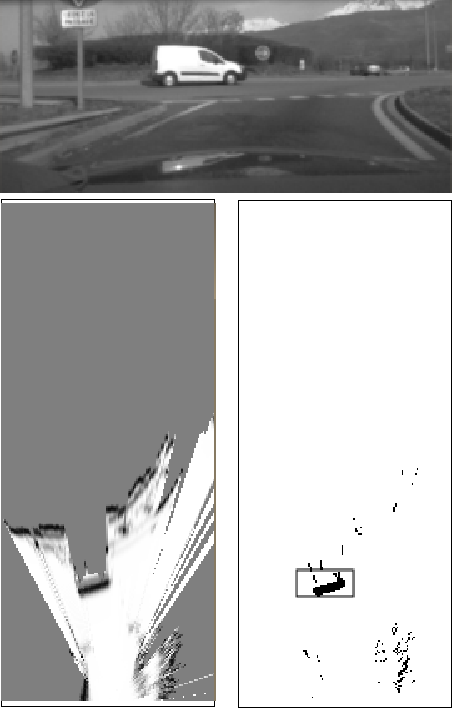
\includegraphics[scale=0.60]{img/fig:result:scenetwocarrondepoint}
     \end{tabular}
   \caption{Car detected in the roundabout}
   \label{fig:result:scenetwocarrondepoint}
\end{figure}

\subsubsection{Two vehicles at high speed}

This footage was made on a motorway at a high speed. On motorways the movement followed by the car is very close to a beeline, due to this characteristic there is no much rotation in this scenario. This produces a better resulting images from our method, as we can see on the Figure~\ref{fig:result:scenetwocarshighway}.

\begin{figure}[H]
   \centering
     \begin{tabular}{lr}
       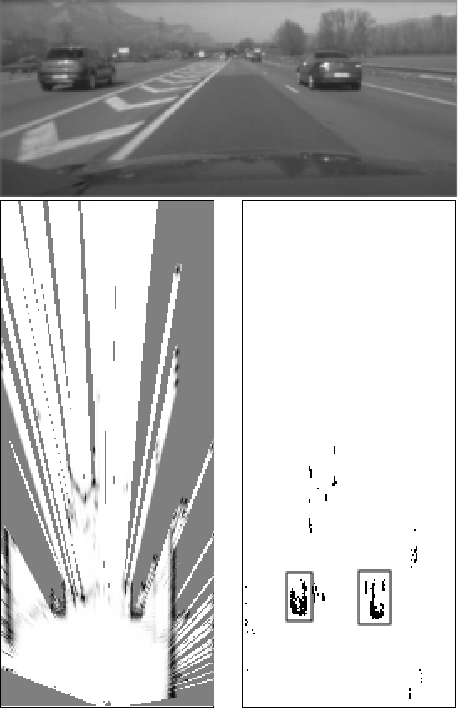
\includegraphics[scale=0.60]{img/fig:result:scenetwocarshighway}
     \end{tabular}
   \caption{Driving in a motorway}
   \label{fig:result:scenetwocarshighway}
\end{figure}

\subsubsection{Completely static scene}

This is the perfect scenario to verify how good our method can be in removing the static environment. In this scenario there is no other moving vehicle on the street, and the vehicle is performing a soft curve to the left Figure~\ref{fig:result:scenestatic}. We can see from the East part, some non dense black dots in the image, but nothing significant, which lead us to assume that there is no moving objects in the scene.

\begin{figure}[H]
   \centering
     \begin{tabular}{lr}
       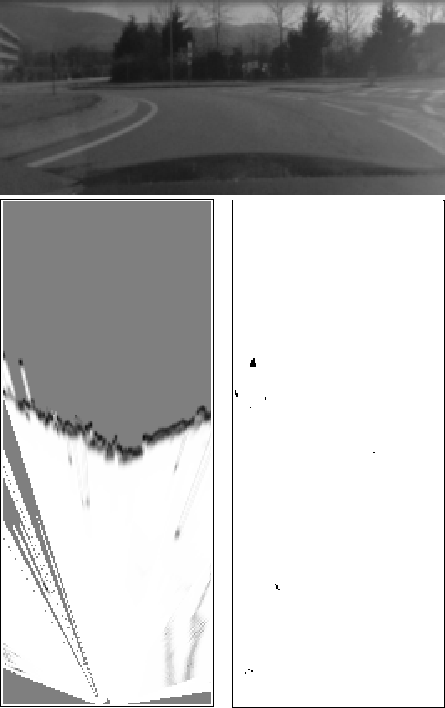
\includegraphics[scale=0.60]{img/fig:result:scenestatic}
     \end{tabular}
   \caption{Driving in an empty road}
   \label{fig:result:scenestatic}
\end{figure}

\section{Conclusion}

\textit{Goal: Express what we can conclude from this work, talk about future work, may be}
